% Diagnosing Candidate-Set and Reranking Failures in Scientific Claim Retrieval:
% A Controlled SciFact Case Study
%
% Venue-neutral manuscript. Standard article class, A4, 11pt, single column.
% Compile with:  latexmk -pdf main.tex     (or:  tectonic main.tex)
%
% ---------------------------------------------------------------------------
% ANONYMOUS MODE
% Set \anonymoustrue below to compile a double-blind version. This replaces the
% author block, the repository URL and the acknowledgement-style statements with
% neutral placeholders. Everything else is unchanged.
% ---------------------------------------------------------------------------

\documentclass[11pt,a4paper]{article}

\newif\ifanonymous
\anonymousfalse   % <-- change to \anonymoustrue for an anonymized submission

% ---------------------------------------------------------------------------
% AFFILIATION AND CONTACT
% Edit these three macros in one place; they are used wherever the author block
% appears. The affiliation is deliberately independent: no institutional
% affiliation is claimed.
% ---------------------------------------------------------------------------
\newcommand{\authorname}{Saqlain Ahmed}
\newcommand{\authoraffiliation}{Independent Researcher}
\newcommand{\authoremail}{saqlainjuna@gmail.com}

% Repository URL used in the reproducibility statement.
% TODO: verify repository availability before submission. The Git remote configured
% for this project is https://github.com/SaqlainXoas/failure-aware-scientific-retrieval
% but that repository was PRIVATE when this manuscript was prepared (2026-08-12), so no
% public-availability claim is made in the text. Make the repository public (or replace
% this with an archival DOI, e.g. Zenodo) and then set \repopublictrue below.
\newif\ifrepopublic
\repopublicfalse
\newcommand{\repourl}{https://github.com/SaqlainXoas/failure-aware-scientific-retrieval}

\usepackage[T1]{fontenc}
\usepackage[utf8]{inputenc}
\usepackage{lmodern}
\usepackage{geometry}
\geometry{a4paper,left=2.4cm,right=2.4cm,top=2.4cm,bottom=2.6cm}
\usepackage{microtype}
\usepackage{amsmath}
\usepackage{amssymb}
\usepackage{graphicx}
\usepackage{booktabs}
\usepackage{array}
\newcolumntype{L}[1]{>{\raggedright\arraybackslash}p{#1}}
\usepackage{caption}
\usepackage[numbers,sort&compress]{natbib}
\usepackage{xcolor}
\usepackage[hidelinks]{hyperref}
\hypersetup{
  colorlinks=true,
  linkcolor=black,
  citecolor=[rgb]{0.10,0.25,0.55},
  urlcolor=[rgb]{0.10,0.25,0.55},
  pdftitle={Diagnosing Candidate-Set and Reranking Failures in Scientific Claim Retrieval: A Controlled SciFact Case Study},
  pdfsubject={Information retrieval; failure analysis; SciFact}
}
\usepackage{url}

\captionsetup{font=small,labelfont=bf,width=0.95\textwidth,skip=6pt}
\setlength{\parskip}{0pt}
\setlength{\parindent}{1.2em}
\setlength{\emergencystretch}{1.5em}
\setlength{\textfloatsep}{12pt plus 2pt minus 3pt}
\setlength{\intextsep}{12pt plus 2pt minus 3pt}
\renewcommand{\arraystretch}{1.05}

% Float placement: allow floats to share pages with text so that wide, short
% figures do not force nearly empty float pages.
\renewcommand{\topfraction}{0.90}
\renewcommand{\bottomfraction}{0.80}
\renewcommand{\textfraction}{0.08}
\renewcommand{\floatpagefraction}{0.80}
\setcounter{topnumber}{3}
\setcounter{bottomnumber}{2}
\setcounter{totalnumber}{4}

\newcommand{\cand}{\ensuremath{\mathrm{candidate\_success}_{50}}}
\newcommand{\fin}{\ensuremath{\mathrm{final\_success}_{10}}}

\title{\bfseries Diagnosing Candidate-Set and Reranking Failures in Scientific Claim
Retrieval: A Controlled SciFact Case Study}

\ifanonymous
  \author{Anonymous Author(s)\\ \small Affiliation withheld for review}
\else
  \author{%
    \authorname\\
    \small \authoraffiliation\\
    \small \href{mailto:\authoremail}{\texttt{\authoremail}}%
  }
\fi

\date{\today}

\begin{document}
\maketitle

\begin{abstract}
\noindent
Retrieval pipelines are usually evaluated with aggregate ranking metrics, which show how often a
pipeline succeeds but not why it fails. A pipeline can fail in two ways: the first stage never
retrieves the relevant document, or it does but the reranker does not rank it highly. We study
this distinction on SciFact by labelling every failed query as one of these two cases. We
evaluate three retrievers --- BM25, a BGE bi-encoder, and their reciprocal rank fusion --- each
followed by the same MS MARCO cross-encoder; all models are frozen. Our results show that fusion gives the
best candidate recall, but final top-10 success increases only from 84.6\% to 87.7\%. The main
change is in the type of failure: the fraction of failures caused by the first stage drops from
76\% to 25\%, while reranking failures become more common. We also find that the cross-encoder
does not significantly improve ranking quality on the held-out split. A logistic model trained on
features from the retrieval output separates failing queries better than the raw reranker score,
but is significantly worse calibrated, so it is more useful for abstention and routing than for
reporting confidence. Overall, better first-stage recall did not lead to a comparable improvement
in final top-10 success, and a larger share of the remaining failures occurred at the reranking
stage. Our findings apply to SciFact and the models we evaluate.
\end{abstract}

\noindent\textbf{Keywords:} information retrieval; failure analysis; scientific claim
verification; cross-encoder reranking; reciprocal rank fusion; query performance prediction;
selective prediction; probability calibration; SciFact.

\section{Introduction}

A two-stage retrieval pipeline can fail in two structurally different ways. Either the first
stage never surfaces the relevant document, in which case the second-stage reranker is
irrelevant to the outcome, or the first stage surfaces it and the reranker fails to place it
near the top. The two situations call for opposite remedies: more candidate recall in the first
case, a better reranker in the second. A single Recall@10 or nDCG@10 figure does not distinguish
them, so two systems with the same headline number can sit one improvement away from very
different ceilings.

We study that distinction on SciFact \citep{wadden2020scifact}, a scientific
claim-verification dataset whose retrieval task is to find the abstract containing the annotated
evidence for a claim. Three questions organize the work:

\begin{enumerate}
  \item How do lexical, dense and hybrid first-stage retrieval compare on candidate recall
        under an otherwise identical pipeline?
  \item When a pipeline fails, is the failure a candidate-set failure or a reranking failure,
        and does that composition change as the first stage improves?
  \item Can a lightweight model, using only signals available at inference time, predict which
        queries will fail better than the reranker's own top score?
\end{enumerate}

The study is narrow by design. No model is fine-tuned, no additional dataset is introduced, and
we do not try to build a stronger retriever. The contribution is a decomposition, a protocol
that keeps its parts separable, and a full accounting of the results, two of which came out
contrary to our working hypothesis.

\paragraph{Contributions.}
\begin{enumerate}
  \item An exhaustive decomposition of multi-stage retrieval failures into
        \emph{candidate-set failures} and \emph{reranking failures}, via a five-way transition
        taxonomy that partitions the query set exactly (Section~\ref{sec:taxonomy}).
  \item A controlled comparison of BM25, a frozen dense bi-encoder and their reciprocal rank
        fusion under a shared candidate depth and a shared frozen reranker
        (Section~\ref{sec:firststage}).
  \item Evidence that, on SciFact, improving candidate recall shifts the composition of the
        remaining failures toward the reranking stage without an equally large improvement in
        final success (Section~\ref{sec:decomposition}).
  \item An evaluation of a frozen general-domain MS MARCO cross-encoder on scientific claims
        reporting only what the data supports: reranking does not reliably improve final
        ranking quality here, and a stronger calibration-set claim of degradation did not
        replicate held out (Sections~\ref{sec:rerank}, \ref{sec:heldout}).
  \item A lightweight inference-time failure-risk model that improves discrimination over the
        raw reranker score while producing significantly worse probability calibration, two
        properties usually reported as one (Section~\ref{sec:risk}).
  \item A leakage-conscious process in which the SciFact test split was opened exactly once,
        after models, features, thresholds and the primary-pipeline rule were fixed
        (Sections~\ref{sec:leakage}, \ref{sec:reproducibility}).
\end{enumerate}

\paragraph{Terminology.}
We use \emph{failure-risk model} (equivalently \emph{risk model} or \emph{lightweight
confidence model}) for the logistic model of Section~\ref{sec:riskmodel}, and reserve
\emph{calibration} for probability calibration in the Brier-score and reliability-diagram
sense. The released artifacts name this model \texttt{common-feature calibrator}; that name is
retained in the repository and in Figure~\ref{fig:reliability} so that every number in this
paper remains traceable to its source file.

\section{Related Work}

\paragraph{SciFact, scientific document retrieval and zero-shot evaluation.}
SciFact frames scientific claim verification as retrieving abstracts that contain evidence for
or against a claim, together with annotated rationales \citep{wadden2020scifact}. Two properties
make it a useful setting here: relevance is defined by \emph{annotated} evidence rather than by
topicality, which sharpens what a retrieval failure means, and an abstract that never enters the
candidate set cannot be recovered downstream, which is the structural asymmetry the
decomposition exploits. Scientific retrieval has motivated domain-specific encoders such as
SPECTER \citep{cohan2020specter}; we use general-domain models throughout and measure domain
transfer instead of engineering around it. SciFact is
accessed through BEIR, a heterogeneous benchmark for zero-shot retrieval evaluation
\citep{thakur2021beir}, whose central finding is that no single paradigm dominates every
collection: reranking pipelines transfer well on average while BM25 remains competitive on
individual datasets. Sections~\ref{sec:rerank} and~\ref{sec:heldout} are a dataset-specific
instance of that variance, not a contradiction of it.

\paragraph{Sparse, dense and hybrid retrieval.}
BM25 remains the standard term-matching baseline \citep{robertson2009bm25}; we use the
\texttt{bm25s} implementation \citep{lu2024bm25s}. Dense bi-encoders embed queries and documents
independently and match in vector space \citep{karpukhin2020dpr}; the encoder used here is
trained with the C-Pack recipe \citep{xiao2024cpack}. The two families fail differently, one on
lexical mismatch and the other on embedding drift, so combining them is common practice.
Reciprocal Rank Fusion (RRF) does so using rank positions instead of raw scores, which spares us
having to reconcile the incompatible scales of BM25 and cosine similarity
\citep{cormack2009rrf}. We use it unmodified and untuned, as a fixed comparator.

\paragraph{Cross-encoder reranking and domain transfer.}
Cross-encoders score a query and a document jointly and are the standard second stage
\citep{nogueira2019passage}, with sequence-to-sequence variants following the same design
\citep{nogueira2020monot5}. Such models are typically trained on MS MARCO
\citep{bajaj2016msmarco}, a general-domain web collection. Section~\ref{sec:rerank} measures how
one such reranker transfers to scientific claims. Because the reranker is frozen, the study
observes the interaction between candidate recall and reranking instead of training a new
end-to-end system.

\paragraph{Query performance prediction, selective prediction and calibration.}
Query performance prediction (QPP) estimates how well a system has done on a query from the
retrieval output alone, without relevance judgments; the pre- and post-retrieval families are
surveyed by \citet{carmel2010querydifficulty}, with clarity-based
\citep{cronentownsend2002clarity} and score-distribution-based \citep{shtok2012querydrift}
predictors as canonical instances. Recent work extends QPP to conversational search
\citep{meng2023qpp} and documents its limits: \citet{chifu2025qpplimits} report that predictor
accuracy varies strongly with collection and ranker and that QPP-driven selective query
processing yields only marginal gains. Our features are in the post-retrieval
score-distribution tradition, but the target differs: we predict the binary event that the final
top ten contains annotated evidence, which is the quantity an abstention policy consumes, and
not a graded effectiveness value. Reporting that model through a risk--coverage curve
places it in the selective-prediction framework, where a system may decline to answer in order
to reduce error on what it does answer \citep{elyaniv2010selective,geifman2017selective}.
Finally, a score can order failures well and still be a poor probability. The raw cross-encoder
logit is not a probability, so our probability baseline is a Platt scaling of it
\citep{platt1999probabilistic} fitted on training data only, and calibration quality is measured
with the Brier score \citep{brier1950verification} and reliability diagrams
\citep{niculescu2005goodprobabilities,guo2017calibration}. Because we keep calibration separate
from ranking quality, Section~\ref{sec:risk} can report an improvement and a degradation for the
same model without contradiction.

\paragraph{Recent overlapping studies.}
Two recent studies overlap directly with this setting and are worth distinguishing carefully.
\citet{aljoofi2026multistage} present a controlled empirical study of multi-stage retrieval for
scientific literature that also combines lexical matching, dense retrieval, RRF fusion and
cross-encoder reranking, and also evaluates on SciFact. Their emphasis is
configuration-level: which pipeline composition performs best, with ablations on
pseudo-relevance feedback and passage pooling, and cross-dataset checks on PubMedQA and
SciDocs. They report cross-encoder reranking as the primary driver of their final gains and
report an RRF ``dilution'' effect in which fusion does not consistently beat the strongest
dense retriever. Our first-stage observation agrees with that second point, since fusion buys
candidate recall at the cost of top-10 precision (Section~\ref{sec:firststage}), while our
reranking result points the other way. The two studies are not directly comparable, because the
encoders, candidate depths, indexing units and reported absolute numbers all differ. We
therefore read the contrast as a reason to report reranker-specific evidence, not as a
refutation of their finding.
\citet{apurba2026sciret} study retrieval and reranking for scientific
retrieval-augmented generation over CORD-19 across corpus scales, and independently observe
that an MS MARCO-trained cross-encoder reduces precision on a scientific corpus. Their
retrieval labels are pseudo-relevance labels derived from their own hybrid system, and the work
is a preprint that has not been peer reviewed, so we cite it as converging but weaker evidence.

\paragraph{How this study differs.}
This paper does not introduce a larger or better retrieval pipeline, and it makes no
state-of-the-art claim. It focuses on the structural decomposition of failures, asking which
stage could possibly have fixed a given failure, instead of ranking configurations. It keeps a
held-out split that is evaluated exactly once under choices fixed in advance, treats failure
discrimination and probability calibration as separate properties, and states which
calibration-set findings replicated on held-out data. These are differences of protocol and
framing on a single small dataset, not claims of novelty in retrieval modelling.

\section{Experimental Design}

\subsection{Dataset and splits}
\label{sec:data}

SciFact is accessed through \texttt{ir\_datasets} as \texttt{beir/scifact}: a corpus of 5{,}183
abstracts, 809 training claims (919 positive judgments) and 300 test claims (339 positive
judgments). Every training and test claim used here has at least one positive relevance
judgment.

The 809 training claims are partitioned 80/20 into 647 \emph{calibration-train} and 162
\emph{calibration-dev} queries by sorting the query identifiers and shuffling with
\texttt{random.Random(42)}. Sorting before shuffling makes the partition independent of the
dataset library's iteration order across versions. The resulting query-identifier files are
committed to the repository, so later work reuses the stored split instead of recomputing it.

The 300-query test split was held out for the entire development of the study and opened
exactly once, at the end, for the evaluation in Section~\ref{sec:heldout}. Sections
\ref{sec:firststage}--\ref{sec:risk} report calibration-set results, which is where every
design decision was made.

\subsection{Retrieval pipelines}
\label{sec:pipelines}

Three first-stage retrievers each return the top 100 abstracts per query over corpus text formed
as \texttt{title$\backslash$n abstract}. \textbf{BM25} runs via \texttt{bm25s}
\citep{lu2024bm25s} with parameters pinned explicitly ($k_1 = 1.5$, $b = 0.75$, $\delta = 0.5$,
Lucene scoring and IDF, lower-casing, English stopwords, token pattern
\texttt{(?u)$\backslash$b$\backslash$w$\backslash$w+$\backslash$b}, no stemmer); these were the
library defaults at the time, and recording them concretely in each run manifest prevents a later
release from silently changing the experiment. \textbf{Dense} uses
\texttt{BAAI/bge-small-en-v1.5} \citep{xiao2024cpack} pinned to revision \texttt{5c38ec7}, with
the model card's query instruction applied to queries only and cosine similarity over normalized
embeddings. \textbf{Hybrid} is Reciprocal Rank Fusion \citep{cormack2009rrf} of the two rankings
with $k = 60$, fixed in advance and never tuned, truncated back to 100 so all three pipelines
emit the same candidate depth.

\subsection{Reranking}
\label{sec:reranking}

All three pipelines are reranked by \texttt{cross-encoder/ms-marco-MiniLM-L6-v2}
\citep{nogueira2019passage,bajaj2016msmarco}, pinned to revision \texttt{c5ee24c}, over that
pipeline's \emph{own} top 50 candidates. No model is fine-tuned. The reranker can only reorder
what its retriever supplied, and that constraint makes the decomposition below well defined.

\subsection{Failure taxonomy}
\label{sec:taxonomy}

For a query $q$ with gold abstracts $G(q)$, first-stage ranking $R_1(q)$ and reranked ranking
$R_2(q)$:
\begin{align}
  \cand(q) &= \mathbf{1}\!\left[\, G(q) \cap R_1(q)_{1:50} \neq \emptyset \,\right], \\
  \fin(q)  &= \mathbf{1}\!\left[\, G(q) \cap R_2(q)_{1:10} \neq \emptyset \,\right].
\end{align}

Each query then receives exactly one of five transition labels. The candidate check is
evaluated first and is the only exit for $\cand = 0$, so a candidate-set failure can never be
mislabelled as a reranker rescue.

\begin{center}
\small
\begin{tabular}{ll}
\toprule
\textbf{Label} & \textbf{Condition} \\
\midrule
\texttt{no\_opportunity}      & gold not in the top-50 candidate set \\
\texttt{already\_successful}  & gold in the top 10 both before and after reranking \\
\texttt{rescued\_by\_reranker}  & gold absent from the first-stage top 10, present after \\
\texttt{degraded\_by\_reranker} & gold present in the first-stage top 10, absent after \\
\texttt{unchanged\_failure}   & gold in the candidate set but in neither top 10 \\
\bottomrule
\end{tabular}
\end{center}

The \textbf{candidate-set failure rate} is the share of all queries labelled
\texttt{no\_opportunity}; the \textbf{reranking failure rate} is the share labelled
\texttt{degraded\_by\_reranker} or \texttt{unchanged\_failure}; the \textbf{final success rate}
is the share labelled \texttt{already\_successful} or \texttt{rescued\_by\_reranker}. These
three quantities partition the query set exactly. Two further quantities are named for their
denominators: \emph{success given opportunity} is final success among queries that had a
candidate-set opportunity, and the \emph{share of failures from the candidate set} is the
fraction of final failures the reranker never had a chance to fix.

\subsection{Failure-risk prediction}
\label{sec:riskmodel}

Eight features are computed per query, all from the pipeline's own output and none from
relevance judgments. Four are first-stage: the top-1 score and the top1--top2 margin, each
min--max normalized within the query's own 50-candidate set; the Spearman correlation between
first-stage and reranked positions; and whether the first-stage top-1 document survives into the
reranked top 3. Within-query normalization lets one feature definition serve BM25 scores, cosine
similarities and RRF fusion scores without a fitted cross-query transform. Four
are reranker-side: the top-1 score, the top1--top2 margin, and the mean and standard deviation
of the top-5 reranker scores.

A \texttt{StandardScaler} followed by \texttt{LogisticRegression} with
\texttt{class\_weight="balanced"} predicts $\fin$. The class weighting was chosen from the 83/17
class imbalance measured on calibration-train, before any development-set result was seen. Two
baselines are reported beside the risk model and kept separate from it: the \textbf{raw reranker
top-1 score}, used for ranking metrics only, since it is not a probability and so no Brier score
is computed for it; and that same score after \textbf{Platt scaling fitted on calibration-train}
\citep{platt1999probabilistic}, which gives the baseline a genuine probability and therefore a
like-for-like Brier score. Platt scaling is monotone, so it leaves AUROC and AUPRC unchanged. A
hybrid-only exploratory ablation adding the BM25/dense top-10 overlap feature is reported
alongside the primary model, and never replaces it.

\subsection{Statistical analysis}
\label{sec:stats}

All comparisons use a paired query-level percentile bootstrap: 1{,}000 resamples, 95\%
intervals, seed 42, with the same resampled query identifiers applied to both sides and the
difference always reported as $B - A$. Resamples that become single-class fall back to the
degenerate-but-defined AUROC/AUPRC value instead of being dropped, which would bias the
interval toward whichever side survives more often. Intervals are reported for a fixed,
pre-specified list of comparisons, not for every possible pair. We describe an interval
that excludes zero as \emph{significant} in this percentile-bootstrap sense; no multiplicity
correction is applied across the comparison list, which is a further reason to read individual
intervals conservatively.

The pre-specified protocol evaluates the risk model on the 162 calibration-dev queries, which
contain only about 20 failures, too few to separate the models. A secondary, higher-powered
estimate therefore pools out-of-fold predictions from stratified 5-fold cross-validation over
all 809 calibration queries, raising the failure count to 117--137 depending on pipeline.
Within each fold the scaler, the logistic regression and the Platt baseline are fitted on that
fold's training portion alone. This changes estimation power, not model selection: thresholds
are still chosen on calibration-dev by the pre-specified rule, the train/dev result is still
reported unchanged, and the test split remains untouched.

\subsection{Leakage controls}
\label{sec:leakage}

The dataset, splits, model identities, candidate depth, failure definitions, primary metrics,
the confidence target, the calibration method and the list of statistical comparisons were fixed
in a project protocol document written before any experiment was executed, and the dated
decisions taken under it are recorded in an experiment log released with the code. We do not
call this a preregistration, since no public, externally verifiable preregistration exists. The
protocol was documented before the experiments ran, and the analysis choices were recorded
before the held-out evaluation.

The operational controls are as follows. The scaler and the logistic regression are fitted on
calibration-train only; abstention thresholds are selected on calibration-dev only; no feature
is derived from relevance judgments; and RRF was never tuned. The primary pipeline for the
risk-model analysis was chosen by a rule fixed in advance, the highest calibration-dev
Recall@50, which picked the hybrid pipeline. Reaching the held-out split requires calling
a separately named loader: the calibration split resolver accepts only the two calibration
split names and raises on anything else, including \texttt{test}, and unit tests assert this,
that no development-set feature value ever reaches a \texttt{fit} call, that cross-validation
predicts each query exactly once out of fold, and that the raw reranker score is never reported
as a probability. Opening the held-out data therefore took an explicit, greppable change to the
code.

\section{Results}

\subsection{First-stage retrieval}
\label{sec:firststage}

Table~\ref{tab:firststage} reports the three first stages on both splits. Fusion buys candidate
recall at the cost of top-10 precision: the hybrid pipeline leads on Recall@50 by 1.8 points
over dense on calibration data and by 1.9 points held out, while trailing dense on nDCG@10 on
both splits. Under the pre-specified selection rule, highest calibration-dev Recall@50, hybrid
is the primary pipeline for the risk-model analysis, and the same rule picks the same pipeline
out of sample.

\begin{table}[tbp]
\centering
\small
\caption{First-stage retrieval before reranking; best value per column and panel in bold. Fusion
leads on Recall@50 on both splits while trailing dense on nDCG@10. Held-out values are 2--5
points lower throughout, as expected for a split never used for any decision.}
\label{tab:firststage}
\begin{tabular}{lrrrrr}
\toprule
Pipeline & Recall@5 & Recall@10 & Recall@50 & MRR@10 & nDCG@10 \\
\midrule
\multicolumn{6}{l}{\emph{Calibration-dev ($n = 162$)}} \\
BM25         & 0.752 & 0.824 & 0.873 & 0.684 & 0.715 \\
Dense (BGE)  & 0.826 & \textbf{0.866} & 0.948 & \textbf{0.744} & \textbf{0.769} \\
Hybrid (RRF) & \textbf{0.828} & 0.864 & \textbf{0.966} & 0.718 & 0.751 \\
\midrule
\multicolumn{6}{l}{\emph{Held-out test ($n = 300$)}} \\
BM25         & 0.719 & 0.774 & 0.869 & 0.631 & 0.662 \\
Dense (BGE)  & \textbf{0.759} & \textbf{0.836} & 0.925 & \textbf{0.682} & \textbf{0.713} \\
Hybrid (RRF) & 0.758 & 0.822 & \textbf{0.944} & 0.667 & 0.700 \\
\bottomrule
\end{tabular}
\end{table}

\subsection{Candidate-set versus reranking failures}
\label{sec:decomposition}

Table~\ref{tab:decomposition} and Figure~\ref{fig:breakdown} give the central result. Moving
from BM25 to hybrid retrieval cuts candidate-set failures by close to a factor of four on
calibration data, from 11.7\% to 3.1\% of all queries, yet final success improves by only 3.1
points, from 84.6\% to 87.7\%. The reason is visible in the last column: the failures changed
category instead of disappearing. Three quarters of BM25's failures are queries the reranker
could not have fixed; only a quarter of the hybrid pipeline's are. Reranking failures rise
correspondingly from 3.7\% to 9.3\% of all queries, as more borderline evidence reaches the
reranker and is not ranked into the top ten.

\begin{table}[tbp]
\centering
\small
\caption{Failure decomposition. The first three columns partition the query set exactly and sum
to 100\% per row. ``Success given opportunity'' conditions on the gold abstract reaching the
candidate set; ``failures from candidate set'' is the share of \emph{final failures} the reranker
never had a chance to fix.}
\label{tab:decomposition}
\begin{tabular}{lrrrrr}
\toprule
 & Candidate-set & Reranking & Final & Success given & Failures from \\
Pipeline & failure & failure & success & opportunity & candidate set \\
\midrule
\multicolumn{6}{l}{\emph{Calibration-dev ($n = 162$)}} \\
BM25         & 11.7\% & 3.7\% & 84.6\% & 95.8\% & 76.0\% \\
Dense (BGE)  & 4.9\%  & 8.0\% & 87.0\% & 91.6\% & 38.1\% \\
Hybrid (RRF) & 3.1\%  & 9.3\% & \textbf{87.7\%} & 90.4\% & 25.0\% \\
\midrule
\multicolumn{6}{l}{\emph{Held-out test ($n = 300$)}} \\
BM25         & 12.3\% & 6.0\%  & 81.7\% & 93.2\% & 67.3\% \\
Dense (BGE)  & 7.0\%  & 9.3\%  & 83.7\% & 90.0\% & 42.9\% \\
Hybrid (RRF) & 5.3\%  & 10.3\% & \textbf{84.3\%} & 89.1\% & 34.0\% \\
\bottomrule
\end{tabular}
\end{table}

\begin{figure}[tbp]
\centering
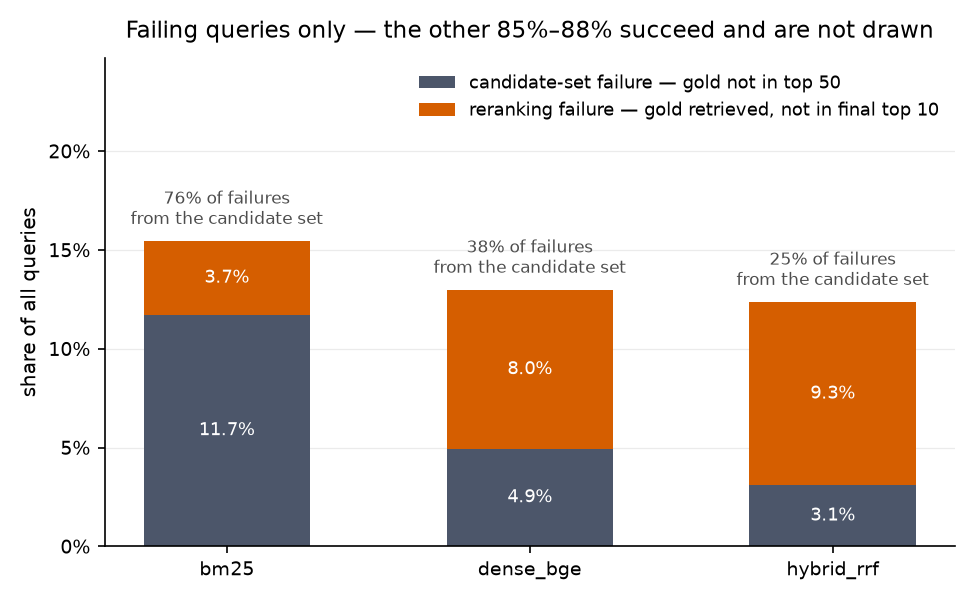
\includegraphics[width=0.66\textwidth]{figures/failure_breakdown.png}
\caption{Failing queries only, on calibration-dev; the successful majority is omitted so the
composition is visible. As candidate recall improves from BM25 to hybrid fusion, the total bar
shrinks modestly while its composition inverts.}
\label{fig:breakdown}
\end{figure}

For this dataset and these models, further first-stage work has little headroom left. The hybrid
pipeline already retrieves annotated evidence into the top 50 for 96.9\% of calibration queries
and 94.7\% of held-out queries, so the binding constraint has moved to the reranking stage.

\subsection{Effect of reranking}
\label{sec:rerank}

Figure~\ref{fig:transitions} shows what reranking actually changed on calibration-dev. The
reranker rescues 5, 4 and 7 queries into the top ten for BM25, dense and hybrid respectively,
and pushes 3, 5 and 6 out of it. Those counts are close to a wash.

\begin{figure}[tbp]
\centering
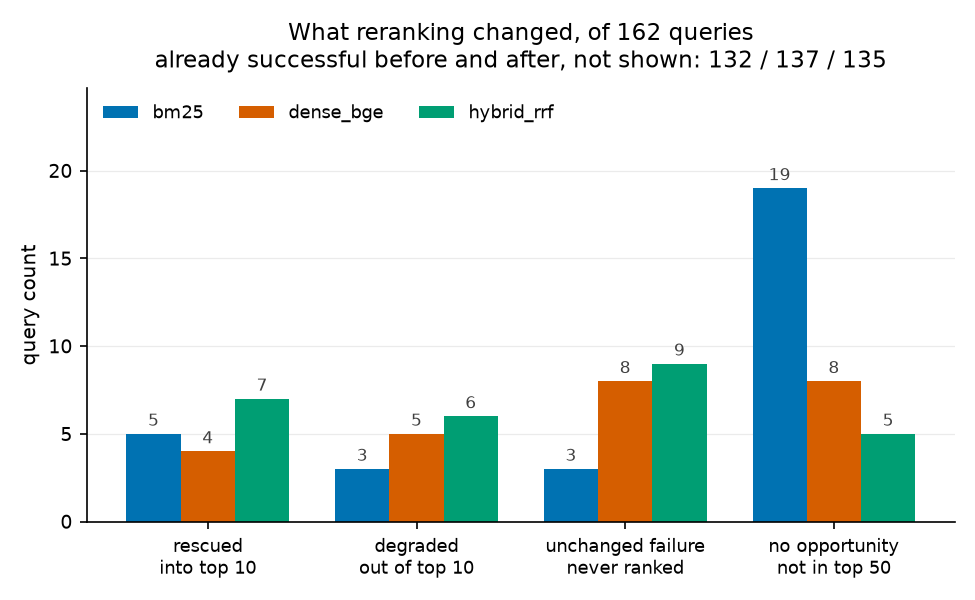
\includegraphics[width=0.66\textwidth]{figures/reranking_transitions.png}
\caption{Transition counts on calibration-dev; queries already successful before and after
reranking (132, 137 and 135 of 162) are omitted. Rescues and degradations are of comparable
magnitude for every pipeline, which is why the aggregate metrics in Table~\ref{tab:rerank}
barely move.}
\label{fig:transitions}
\end{figure}

Table~\ref{tab:rerank} gives the paired before/after differences with bootstrap intervals.
Recall@10 changes are small and every interval crosses zero on both splits. On calibration data
nDCG@10 falls for all three pipelines and the dense interval lies entirely below zero; on
held-out data no before/after comparison is significant for any pipeline, and BM25 nDCG@10
actually rises. The mechanism behind the calibration-set drop is visible in the transition
counts: a rescue typically moves a document into a mid-top-10 position, whereas a degradation
removes a document that was already ranked highly, so degradations cost more nDCG than rescues
recover even when the counts balance.

\begin{table}[tbp]
\centering
\small
\caption{Effect of reranking: paired query-level differences (after $-$ before) with 95\%
percentile bootstrap intervals (1{,}000 resamples, seed 42). Bold marks the single interval
excluding zero; it did not replicate held out.}
\label{tab:rerank}
\begin{tabular}{lrcrc}
\toprule
 & \multicolumn{2}{c}{Recall@10} & \multicolumn{2}{c}{nDCG@10} \\
\cmidrule(lr){2-3}\cmidrule(lr){4-5}
Pipeline & $\Delta$ & 95\% CI & $\Delta$ & 95\% CI \\
\midrule
\multicolumn{5}{l}{\emph{Calibration-dev ($n = 162$)}} \\
BM25         & $+0.015$ & $[-0.019, +0.049]$ & $-0.001$ & $[-0.039, +0.036]$ \\
Dense (BGE)  & $+0.001$ & $[-0.037, +0.038]$ & $\mathbf{-0.044}$ & $\mathbf{[-0.081, -0.009]}$ \\
Hybrid (RRF) & $+0.006$ & $[-0.040, +0.049]$ & $-0.026$ & $[-0.062, +0.010]$ \\
\midrule
\multicolumn{5}{l}{\emph{Held-out test ($n = 300$)}} \\
BM25         & $+0.027$ & $[-0.005, +0.060]$ & $+0.022$ & $[-0.008, +0.052]$ \\
Dense (BGE)  & $-0.013$ & $[-0.043, +0.018]$ & $-0.017$ & $[-0.043, +0.012]$ \\
Hybrid (RRF) & $+0.007$ & $[-0.030, +0.041]$ & $-0.004$ & $[-0.034, +0.024]$ \\
\bottomrule
\end{tabular}
\end{table}

The claim this study supports is therefore the weaker one: for the evaluated MS MARCO
cross-encoder on SciFact, reranking does not reliably improve final ranking quality, and the
stronger statement that it degrades dense retrieval is not supported once held-out data is
taken into account. This is a transfer result about one general-domain reranker applied
unmodified to scientific claims, and it says nothing about cross-encoders as a class. The
converging observation of \citet{apurba2026sciret} on a different scientific corpus is likewise
about transfer.

\subsection{Failure-risk prediction}
\label{sec:risk}

Under the pre-specified train/dev protocol, every raw-versus-model interval crossed zero: with
roughly 20 failures among 162 queries, the comparison was underpowered rather than null. On
calibration-dev the risk model reached AUROC 0.851 against 0.804 for the raw score on the
hybrid pipeline, with a Brier score of 0.166 against 0.097 for the Platt-scaled baseline. The
cross-validated estimate over 809 calibration queries (Table~\ref{tab:risk}) resolves the
comparison in both directions.

\begin{table}[tbp]
\centering
\small
\caption{Failure-risk prediction. \emph{Top panel}: cross-validated over all 809 calibration
queries (pooled out-of-fold predictions from stratified 5-fold cross-validation; 117--137
failures depending on pipeline). \emph{Bottom panel}: the single held-out evaluation (300
queries, roughly 50 failures), with models fitted on calibration-train and never refitted.
Differences are model $-$ baseline with 95\% paired bootstrap intervals; AUROC and AUPRC compare
against the raw reranker score, Brier against the train-fitted Platt scaling of that score.
Higher is better for AUROC and AUPRC; \emph{lower} is better for Brier, so the Brier rows are
unfavourable to the risk model. Bold marks intervals excluding zero.}
\label{tab:risk}
\footnotesize
\begin{tabular}{llrrrc}
\toprule
Pipeline & Metric & Baseline & Risk model & Difference & 95\% CI \\
\midrule
\multicolumn{6}{l}{\emph{Cross-validated over calibration queries ($n = 809$)}} \\
BM25         & AUROC & 0.781 & 0.846 & $\mathbf{+0.065}$ & $\mathbf{[+0.034, +0.098]}$ \\
Dense (BGE)  & AUROC & 0.757 & 0.840 & $\mathbf{+0.083}$ & $\mathbf{[+0.039, +0.124]}$ \\
Hybrid (RRF) & AUROC & 0.758 & 0.827 & $\mathbf{+0.069}$ & $\mathbf{[+0.034, +0.105]}$ \\
BM25         & AUPRC & 0.936 & 0.962 & $\mathbf{+0.025}$ & $\mathbf{[+0.011, +0.043]}$ \\
Dense (BGE)  & AUPRC & 0.940 & 0.965 & $\mathbf{+0.025}$ & $\mathbf{[+0.010, +0.042]}$ \\
Hybrid (RRF) & AUPRC & 0.939 & 0.962 & $\mathbf{+0.023}$ & $\mathbf{[+0.009, +0.039]}$ \\
BM25         & Brier & 0.115 & 0.163 & $\mathbf{+0.048}$ & $\mathbf{[+0.031, +0.065]}$ \\
Dense (BGE)  & Brier & 0.110 & 0.162 & $\mathbf{+0.052}$ & $\mathbf{[+0.032, +0.071]}$ \\
Hybrid (RRF) & Brier & 0.113 & 0.171 & $\mathbf{+0.058}$ & $\mathbf{[+0.039, +0.076]}$ \\
\midrule
\multicolumn{6}{l}{\emph{Held-out test split ($n = 300$), evaluated once}} \\
BM25         & AUROC & 0.767 & 0.811 & $+0.044$ & $[-0.005, +0.092]$ \\
Dense (BGE)  & AUROC & 0.783 & 0.831 & $+0.049$ & $[-0.017, +0.120]$ \\
Hybrid (RRF) & AUROC & 0.750 & 0.784 & $+0.034$ & $[-0.028, +0.102]$ \\
BM25         & AUPRC & 0.937 & 0.951 & $+0.014$ & $[-0.003, +0.032]$ \\
Dense (BGE)  & AUPRC & 0.947 & 0.960 & $+0.014$ & $[-0.007, +0.036]$ \\
Hybrid (RRF) & AUPRC & 0.942 & 0.949 & $+0.007$ & $[-0.012, +0.027]$ \\
BM25         & Brier & 0.131 & 0.179 & $\mathbf{+0.048}$ & $\mathbf{[+0.018, +0.078]}$ \\
Dense (BGE)  & Brier & 0.113 & 0.166 & $\mathbf{+0.054}$ & $\mathbf{[+0.024, +0.084]}$ \\
Hybrid (RRF) & Brier & 0.119 & 0.194 & $\mathbf{+0.075}$ & $\mathbf{[+0.043, +0.107]}$ \\
\bottomrule
\end{tabular}
\end{table}

The risk model discriminates better on all three pipelines and is calibrated worse on all
three. AUPRC deserves a caveat: it is bounded below by the positive class rate, which is 0.852
on the pooled hybrid data, not 0.5. Measured against that floor, the raw score captures
0.088 and the risk model 0.110, so the $+0.023$ difference is roughly a 25\% relative
improvement in the informative part of AUPRC, not the $\sim$2\% the bare numbers suggest. The released artifacts report \texttt{base\_rate} and \texttt{auprc\_over\_base\_rate}
for this reason.

\begin{figure}[tbp]
\centering
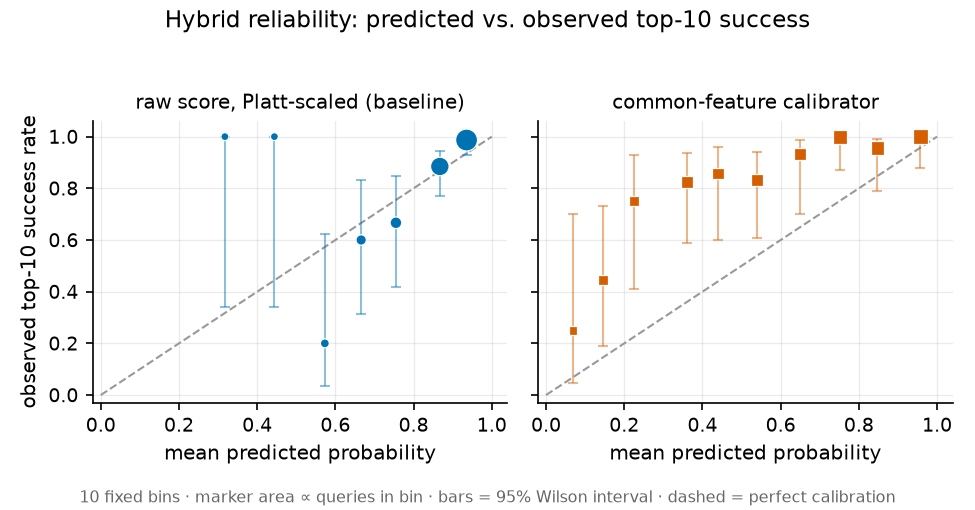
\includegraphics[width=0.76\textwidth]{figures/hybrid_reliability.png}
\caption{Reliability for the hybrid pipeline on calibration-dev. The panel labelled
\emph{common-feature calibrator} is the failure-risk model of Section~\ref{sec:riskmodel}; the
artifact name is kept for traceability. Its points lie above the diagonal in nearly every bin,
so it systematically understates success probability; the Platt-scaled baseline never predicts
below 0.3, leaving its first three bins empty.}
\label{fig:reliability}
\end{figure}

Figure~\ref{fig:reliability} shows the mechanism. The risk model's points lie above the
diagonal at nearly every bin: it systematically understates the probability of success. This is
a direct consequence of \texttt{class\_weight="balanced"}, which up-weights the minority failure
class and pulls predicted probabilities down. That setting was fixed in advance from the
training-split class imbalance; it was not revised after the Brier result appeared, and no
unweighted variant is reported, because selecting one post hoc would convert a pre-specified
choice into a tuned one. The same wider spread of predictions explains both results: more
separation between queries improves the ranking metrics, and pushing predictions toward the
extremes costs the model on Brier.

\begin{figure}[tbp]
\centering
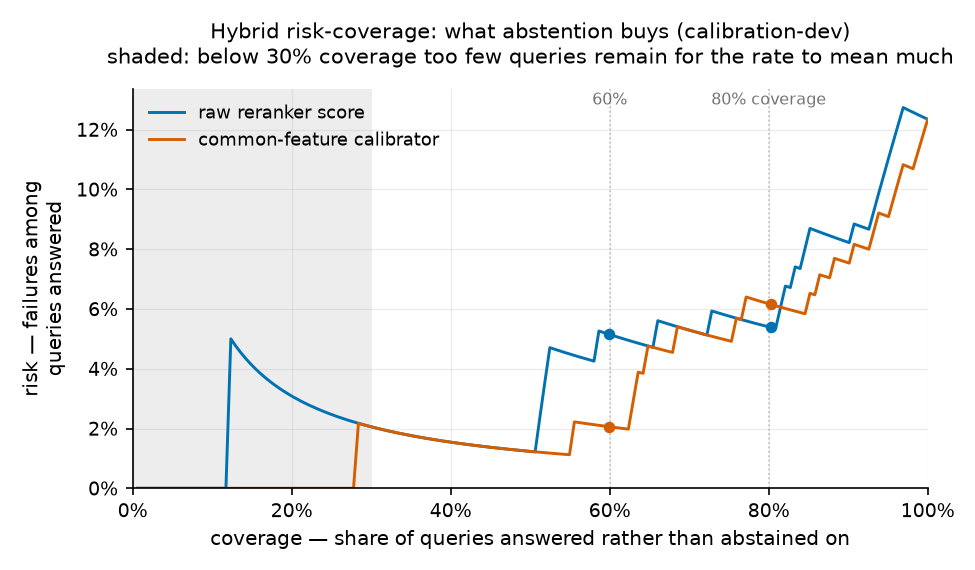
\includegraphics[width=0.68\textwidth]{figures/hybrid_risk_coverage.png}
\caption{Risk--coverage for the hybrid pipeline on calibration-dev. Risk is the failure rate
among answered queries; coverage is the share of queries answered instead of abstained on. The shaded
region (below 30\% coverage) holds too few queries for the rate to be informative. The risk
model's advantage appears where abstention is aggressive.}
\label{fig:riskcoverage}
\end{figure}

The model is therefore usable for \emph{ordering} queries by risk (routing, abstention, triage),
but not for reporting a probability to a user. Figure~\ref{fig:riskcoverage} makes
the operating range concrete: on calibration-dev, answering only the 60\% of queries the risk
model is most confident about raises success from 87.7\% to 97.9\%, against 94.8\% at the same
coverage under the raw score, while at 80\% coverage the two are within a point of each other
(93.8\% versus 94.6\%). The cross-validated pool shows the same pattern with more queries behind
it: 95.9\% against 93.0\% at 60\% coverage.

\subsection{Held-out evaluation}
\label{sec:heldout}

The test split was opened once, after Sections \ref{sec:firststage}--\ref{sec:risk} were
complete and every model, feature and threshold was fixed. The risk models are the
calibration-train models used unchanged; the abstention thresholds are those selected on
calibration-dev. Nothing was refitted and no configuration was altered in response to any
result below.

The lower panel of Table~\ref{tab:risk} reports the held-out risk-model metrics and
Table~\ref{tab:replication} summarizes which calibration-set findings replicated. Four points
stand out.

First, the primary-pipeline rule survives out of sample: hybrid again has the highest Recall@50
(Table~\ref{tab:firststage}). Second, the composition shift replicates with the same ordering
and a smaller spread (Table~\ref{tab:decomposition}). Third, the pipeline comparison is
\emph{stronger} held out: the hybrid pipeline's final success exceeds BM25's by $+0.027$ with a
95\% interval of $[+0.003, +0.050]$, where the corresponding calibration interval had merely
touched zero ($+0.031$, $[+0.000, +0.068]$). Fourth, the significant dense reranking
degradation of Section~\ref{sec:rerank} did not replicate.

For the risk model, the calibration failure replicates decisively, with the Brier degradation
significant on every pipeline and every split tested, while the discrimination advantage
replicates only in direction. All three held-out AUROC differences are positive and none is
individually significant at 300 queries holding roughly 50 failures; this is the same power
limitation that made the pre-specified calibration-dev comparison inconclusive, and the reason
the cross-validated estimate exists. Held-out data agrees in direction with that estimate
without being able to confirm it on its own.

\begin{table}[tbp]
\centering
\small
\caption{Replication summary. Where a held-out result contradicted a calibration-set result, the
calibration-set claim was weakened rather than the reverse.}
\label{tab:replication}
\footnotesize
\begin{tabular}{L{4.4cm}L{3.3cm}L{3.5cm}L{2.6cm}}
\toprule
Finding & Calibration & Held-out & Replicated? \\
\midrule
Best Recall@50 & hybrid, 0.966 & hybrid, 0.944 & Yes; selection rule holds out of sample \\
Share of failures from candidate set & $76\% \to 25\%$ & $67\% \to 34\%$ & Yes; same ordering and direction \\
Hybrid vs.\ BM25 final success & $+0.031$, CI touches 0 & $+0.027$, CI $[+0.003, +0.050]$ & Yes, and stronger held out \\
Reranking degrades dense nDCG@10 & $-0.044$, CI $[-0.081, -0.009]$ & $-0.017$, CI $[-0.043, +0.012]$ & \textbf{No} \\
Risk-model Brier worse than Platt & $+0.048$ to $+0.058$ (CV) & $+0.048$ to $+0.075$ & Yes; significant on all three \\
Risk-model AUROC better than raw & $+0.065$ to $+0.083$ (CV) & $+0.034$ to $+0.049$, CIs cross 0 & Direction yes, power no \\
\bottomrule
\end{tabular}
\end{table}

\subsection{Threshold transfer}
\label{sec:threshold}

Held-out data also answers an operational question the calibration split cannot: whether an
abstention threshold chosen on calibration-dev still delivers its intended coverage on unseen
queries. Table~\ref{tab:threshold} carries the hybrid thresholds over unchanged.

\begin{table}[tbp]
\centering
\small
\caption{Threshold transfer for the hybrid pipeline. Each cutoff was selected on calibration-dev
to hit the target coverage, then applied unchanged to the 300 held-out queries; ``achieved'' is
the share of held-out queries kept.}
\label{tab:threshold}
\begin{tabular}{lrrrr}
\toprule
 & \multicolumn{2}{c}{Raw reranker score} & \multicolumn{2}{c}{Failure-risk model} \\
\cmidrule(lr){2-3}\cmidrule(lr){4-5}
Target coverage & Achieved & Success rate & Achieved & Success rate \\
\midrule
100\% & 99.7\% & 0.846 & 98.0\% & 0.857 \\
80\%  & 74.0\% & 0.892 & 71.7\% & 0.916 \\
60\%  & 48.3\% & 0.952 & 58.0\% & 0.931 \\
\bottomrule
\end{tabular}
\end{table}

At the aggressive setting the risk model's cutoff transferred more consistently: it landed
within two points of its 60\% target where the raw score undershot by roughly twelve points.
The narrow reading is the right one. The risk model's \emph{score distribution}, and with it the
selected cutoff, kept its shape better across these two splits. In absolute terms its
probabilities remain poorly calibrated, as the Brier results in Table~\ref{tab:risk} show.
Threshold
transfer and probability calibration are different properties, and only the former is supported
here. It is also a single observation on one split, at one operating point, for one pipeline.

\section{Qualitative Failure Analysis}
\label{sec:qualitative}

Twelve hybrid calibration-dev queries were selected by fixed rules before any case text was
read: the two highest-confidence incorrect queries first, then evenly spaced confidence
quantiles within each transition category, with query identifier as a stable tie-break. The
selection is recorded as a machine-readable artifact so that it cannot be retrofitted to the
narrative. The counts below describe those twelve cases and are not estimates of population
frequency.

Four failure modes recur. \textbf{Evidence outside the cutoff} (7 of 12 cases) is the most
common: the annotated abstract exists in the corpus and is topically adjacent but never enters
the top 50. \textbf{Terminology mismatch} (4) covers claims phrased in one register, such as
``increased flux of microbial products'', whose annotated evidence is written in another, here
in terms of intestinal barrier compromise. \textbf{Lexical distraction} (4)
covers claims combining two concepts where one dominates retrieval: a claim about
ischemia-reperfusion \emph{in aging} retrieves ischemia papers and misses the aging study.
\textbf{Cross-encoder overconfidence} (3) covers the reranker's preference for near-verbatim
title matches. In the single highest-confidence error, an abstract naming ``B cells'',
``exhaustion'' and ``HIV'' in its title is scored 3.97 while every other candidate falls below
zero, and the annotated review, which discusses antibody responses more broadly, stays below the
cutoff.

The two rescues are informative in the opposite direction. In one, the first stage is distracted
by generic inhibitor language and the reranker recognises the exact compound and mechanism
strongly enough to pull the annotated document into the top ten. Pairwise scoring does add
something on this data, but it gives back about as much as it gains.

A caveat applies throughout: SciFact marks \emph{annotated} evidence, not the complete set of
scientifically relevant abstracts. Several cases counted here as failures are abstracts a domain
reader might well call relevant but which were not the annotated source. The risk model therefore
predicts retrieval of annotated evidence, not scientific correctness, and the rates in
Table~\ref{tab:decomposition} should be read the same way.

\section{Discussion}

The decomposition changes what an aggregate number means. Read only through final success, the
hybrid pipeline is a three-point improvement over BM25 on calibration data and a 2.6-point
improvement held out; read through the decomposition, it nearly eliminates one failure mode
while a second grows to partially replace it. A practitioner who saw only the aggregate might
invest in a better first stage; the decomposition says that on SciFact, with these models, that
investment has little headroom left.

That reading depends on the second result. Under the evaluated frozen models, the standard
second stage does not reliably improve final ranking quality here: rescues and degradations are
of comparable magnitude, and no held-out before/after comparison is significant. Applying a
general-domain MS MARCO cross-encoder unmodified to scientific claims carries a cost in this
setting. This is consistent with BEIR's observation that no single paradigm
dominates every collection \citep{thakur2021beir}, and it stands in apparent tension with
\citet{aljoofi2026multistage}, who report reranking as the primary driver of gains on SciFact
under a different pipeline configuration. Resolving that tension would require holding the
reranker, the candidate depth and the indexing unit fixed across both setups, which we have not
done.

The third result concerns what ``confidence'' means operationally. One lightweight model is
better than the raw reranker score at ordering queries by risk and worse than a one-parameter
Platt baseline at stating the probability that a query will succeed; both directions are
significant in the cross-validated estimate, and the calibration degradation is significant
held out as well. For a routing or abstention system, which consumes an ordering and a cutoff,
that trade is often acceptable; for anything that displays a confidence number to a user, it is
not. Because the class weighting responsible for the compression was fixed in advance and never
revised, we report the trade instead of tuning it away. That also means the attribution to class
weighting is an interpretation supported by the reliability diagram, not a measured ablation.

Finally, the protocol is part of what the study offers. Because the failure definitions, leakage
rules, metrics and comparison list were all fixed before any run existed, the non-replication in
Section~\ref{sec:heldout} is reportable instead of embarrassing: the dense reranking comparison
was specified in advance, so its calibration-set result could not be quietly dropped once
held-out data disagreed.

\section{Limitations}
\label{sec:limitations}

\paragraph{One dataset, and a small one.} SciFact has 5{,}183 abstracts, 162 calibration-dev
queries and 300 held-out queries. Nothing here establishes that the composition shift, or any
other result, generalizes to other collections, domains or corpus sizes. Every claim is scoped
to SciFact under the evaluated models.

\paragraph{Small failure counts.} Roughly 20 failures in the development split made the
pre-specified risk-model comparison inconclusive and motivated the cross-validated secondary
analysis; roughly 50 held-out failures are why the held-out AUROC comparison is directionally
consistent but not individually significant. Development-only intervals should be read as
underpowered rather than as evidence of no effect, and no multiplicity correction is applied
across the pre-specified comparison list.

\paragraph{Off-the-shelf, frozen models.} The reranking result is evidence about
MS MARCO $\rightarrow$ SciFact transfer for one specific cross-encoder, not about cross-encoders
in general; a domain-adapted reranker might behave very differently. RRF likewise ran at
$k = 60$ untuned, so the hybrid pipeline is a fixed comparator, not an optimized system.

\paragraph{One risk-model configuration.} The Brier degradation is consistent with the
pre-specified class weighting, but no unweighted ablation was run, so that attribution is an
interpretation rather than a measurement.

\paragraph{Annotated evidence is not scientific truth.} A topically excellent non-annotated
abstract counts as a failure in these tables, and Section~\ref{sec:qualitative} shows concrete
instances. The risk model's target is retrieval of annotated evidence, not the correctness of a
claim.

\paragraph{The held-out split is spent.} It was evaluated once, as designed, and will not be
used again, so no untouched replication set remains within SciFact. A future change to this
pipeline would need a new dataset, or a new split protocol, to be validated comparably.

\paragraph{One claim was weakened by held-out data.} The dense reranking degradation is reported
in Section~\ref{sec:rerank} because that is what the calibration data showed and because the
protocol fixed that comparison in advance; Section~\ref{sec:heldout} records that it did not
replicate. The calibration-set effect sizes throughout should be read as the optimistic end of
the range.

\section{Conclusion}

Decomposing retrieval failure changes what aggregate metrics mean. On SciFact, under frozen
general-domain models, hybrid fusion looks like a modest three-point improvement in final top-10
success over BM25; the decomposition shows that it nearly eliminates candidate-set failures while
reranking failures grow to partially replace them, leaving the reranking stage as the binding
constraint. That shift replicates on a held-out split evaluated once. For the evaluated
MS MARCO cross-encoder, reranking does not reliably improve final ranking quality here. Failure
also turns out to be predictable from retrieval-internal signals alone: a lightweight risk model
orders at-risk queries better than the reranker's own score and carries an abstention cutoff
across splits more consistently, while stating significantly worse-calibrated probabilities than
a one-parameter Platt baseline.

Two of these results are negative. A fourth, that reranking significantly degrades dense
retrieval, appeared on calibration data and did not survive held-out evaluation; we report it as
not replicating instead of dropping it quietly. The findings belong to SciFact and to the models
evaluated here. What we would expect to carry over is the diagnostic itself, not its numbers.

\section{Reproducibility Statement}
\label{sec:reproducibility}

The code, pipeline configurations, committed split files, result tables, figures and run
manifests underlying every number in this paper are maintained in the project repository.%
\ifrepopublic
\ It is available at \url{\repourl}.
\else
\ The repository was not public at the time of writing; the URL will be stated once it is
released or archived.
\fi
\ Tables and figures are regenerated from saved run artifacts by a single command; no number in
this manuscript was computed by hand, and each was checked against the corresponding committed
JSON or Markdown result file.

Model identities and revisions are pinned where the artifacts support it: the dense encoder at
revision \texttt{5c38ec7} and the cross-encoder at \texttt{c5ee24c} (full 40-character hashes are
recorded in every run manifest), with BM25 parameters recorded explicitly in
each run manifest. Every committed result traces to a run directory, a Git commit hash and a
model revision through the stored manifests; the manifests also record whether the working tree
was clean at run time, and the calibration runs backing Sections
\ref{sec:firststage}--\ref{sec:risk} were executed from a clean tree. Per-query run directories,
cached embeddings and model weights are not committed, as they are regenerable; the commands to
regenerate them are documented in the repository.

The held-out test split was evaluated exactly once, after the retrieval implementations,
configurations, features, models, thresholds and the primary-pipeline selection rule were all
fixed, and nothing was refitted or altered in response to the result. Consequently the SciFact
test split is now \emph{spent} for this line of work: it can no longer serve as untouched
validation data for future modifications of this system, and no independent replication set
remains available within SciFact.

The protocol document that fixed the dataset, splits, models, failure taxonomy, leakage rules
and statistical comparisons was written before any experiment was executed, and the dated
decisions taken under it, including those made after seeing unfavourable results, are recorded
in the repository's experiment log. This is a documented internal protocol and not a public
preregistration.

\bibliographystyle{plainnat}
\bibliography{references}

\end{document}
